\textit{Mars Exploration Rovers} (MER) est une mission de la NASA qui cherche à étudier le rôle joué par l’eau dans
l’histoire de la planète Mars. Deux robots géologues, Spirit et Opportunity (figure 1), se sont posés sur cette
planète, sur deux sites opposés, en janvier 2004. Leur mission est de rechercher et d’analyser différents types de
roches et de sols qui peuvent contenir des indices sur la présence d’eau. 
%Ils sont équipés de six roues et d’une
%suspension spécialement conçue pour leur permettre de se déplacer quelle que soit la nature du terrain rencontré.
%Leur cahier des charges prévoyait une durée de vie de 90 jours martiens (le jour martien est environ 40 minutes
%plus long que le jour terrestre). Spirit a cessé d’émettre le 22 mars 2010, soit 2210 jours martiens après son
%arrivée sur la planète. Début 2017, Opportunity est toujours en activité et il a parcouru plus de 44 km sur Mars.

\begin{figure}[H]
\centering
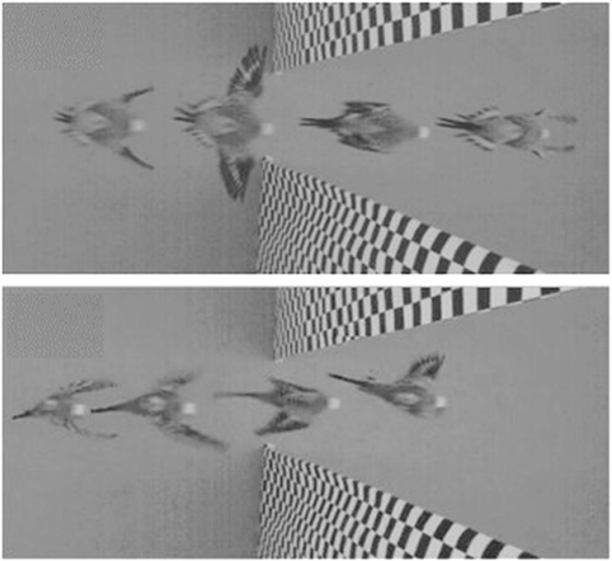
\includegraphics[width=.5\linewidth]{fig_01}
\caption{Vue d’artiste d’un robot géologue de la mission Mars Exploration Rovers (NASA/JPL – Caltech/
Cornell) \label{fig_01}}
\end{figure}



Chaque robot est équipé de plusieurs instruments d’analyse (caméra, microscope, spectromètres) et d’un bras
qui permet d’amener les instruments au plus près des roches et sols dignes d’intérêt. À partir de photographies de
la surface de la planète, prises à plusieurs longueurs d’ondes par différents satellites et par le robot lui-même, les
scientifiques de la NASA définissent une liste d’emplacements (\textit{points d’intérêt} ou PI) où effectuer des analyses.

Cette liste est transmise au robot qui doit se rendre à chaque emplacement indiqué et y effectuer les analyses
prévues. Chaque robot est capable d’effectuer un certain nombre de types d’analyses géologiques correspondant
aux différents instruments dont il dispose. Une fois tous les points d’intérêts visités et les résultats des analyses
transmis à la Terre, le robot reçoit une nouvelle liste de points d’intérêts et démarre une nouvelle exploration.
Compte-tenu des contraintes de transmission entre la Terre et les robots (latence, périodes d’ombre, faible débit,
etc.) il est prévu que les robots travaillent en autonomie pour planifier le parcours de chaque exploration. Ainsi,
une fois la liste des points d’intérêt reçue, le robot analyse le terrain afin de détecter d’éventuels obstacles et
détermine le meilleur chemin lui permettant de visiter l’ensemble de ces points en dépensant le moins d’énergie
possible.

%Après s’être intéressé à l’enregistrement des explorations, des points d’intérêts correspondants et des analyses
%à y mener, ce sujet aborde trois algorithmes qui peuvent être utilisés par le robot pour déterminer le meilleur
%parcours lui permettant de visiter chaque point d’intérêt une et une seule fois. Pour cela nous faisons quelques
%hypothèses simplificatrices.
%\begin{itemize}
%\item La zone d’exploration est dépourvue d’obstacle : le robot peut rejoindre directement en ligne droite n’importe
%quel point d’intérêt.
%\item Le sol est horizontal et de nature constante : l’énergie utilisé pour se déplacer entre deux points ne dépend
%que de leur distance, autrement dit le meilleur chemin est le plus court.
%\item La courbure de la planète est négligée compte tenu de la dimension réduite de la zone d’exploration : nous
%travaillerons en géométrie euclidienne et les points d’intérêts seront repérés par leurs coordonnées cartésiennes
%à l’intérieur de la zone d’exploration.
%\end{itemize}

%Les seuls langages de programmation autorisés dans cette épreuve sont Python et SQL. 
Toutes les questions
sont indépendantes. Néanmoins, il est possible de faire appel à des fonctions ou procédures créées dans d’autres
questions. Dans tout le sujet on suppose que les bibliothèques math, numpy et random ont été importées grâce
aux instructions
\begin{lstlisting}
import math
import numpy as np
import random
\end{lstlisting}
% Si les candidats font appel à des fonctions d’autres bibliothèques ils doivent préciser les instructions d’importation
% correspondantes.

Ce sujet utilise la syntaxe des annotations pour préciser le types des arguments et du résultat des fonctions à
écrire. Ainsi
\texttt{def maFonction(n:int, x:float, d:str) -> np.ndarray:}
signifie que la fonction \texttt{maFonction} prend trois arguments, le premier est un entier, le deuxième un nombre à
virgule flottante et le troisième une chaine de caractères et qu’elle renvoie un tableau numpy.
Une liste de fonctions utiles est donnée à la fin du sujet.


\section{Création d’une exploration et gestion des points d’intérêt}

Une exploration est un ensemble de points d’intérêts à l’intérieur d’une zone géographique limitée, une série
d’analyses étant associée à chaque point d’intérêt. Chaque type d’analyse que le robot peut effectuer est codifié
et référencé par un nombre entier. Un point d’intérêt est repéré par deux entiers, positifs ou nuls, correspondant
à ses coordonnées cartésiennes en millimètres à l’intérieur de la zone d’exploration. L’ensemble des points
d’intérêts d’une exploration qui en contient $n$ est représenté par un objet de type 
%\texttt{numpy.ndarray}, 
\texttt{list}, 
à éléments
entiers, à 2 colonnes et $n$ lignes, l’élément d’indice \texttt{i,0} correspondant à l’abscisse du point d’intérêt $i$ et l’élément
d’indice \texttt{i,1} à son ordonnée.

\begin{figure}[H]
\centering
\begin{tabular} {c||cc} 

 	& x 		& y     \\ \hline 
0 	& 345 	& 635 \\ %\hline 
1 	& 1076 	& 415 \\ %\hline 
2 	& 38 		& 859 \\ %\hline 
3 	& 121 	& 582 \\ %\hline 
\end{tabular}
\caption{Exemple d’exploration avec quatre points d’intérêt \label{fig_02}}
\end{figure}

\subsection{Génération d’une exploration d’essai}
\subsubsection{Choix de points au hasard}
\question{Afin de disposer de données pour tester les différents algorithmes de calcul de chemin qui seront développés plus tard, écrire une fonction qui construit une exploration au hasard. Cette fonction d’entête
\texttt{def générer\_PI(n:int, cmax:int) -> np.ndarray}  
prend en paramètres le nombre de points d’intérêts à générer et la largeur de la zone d’exploration (supposée
carrée) et renvoie un objet de type \texttt{list} %numpy.ndarray 
contenant les coordonnées de $n$ points deux à deux
distincts choisis au hasard dans la zone d’exploration (\autoref{fig_02}).}

\question{Quelles contraintes doivent vérifier les arguments de la fonction \texttt{générer\_PI} ?}

\subsubsection{Calcul des distances}
On dispose de la fonction d’entête \texttt{def position\_robot() -> tuple} qui renvoie un couple donnant les coordonnées actuelles du robot dans le système de coordonnées de l’exploration
à planifier. Ainsi l’instruction \texttt{x, y = position\_robot()} permet de récupérer les coordonnées courantes du
robot.
Afin de faciliter l’application des différents algorithmes de recherche de chemin, on souhaite construire un tableau
des distances entre les différents points d’intérêt d’une exploration et entre ceux-ci et la position courante du
robot au moment du calcul.

\question{Écrire une fonction d’entête \texttt{def calculer\_distances(PI:list) -> list:} %\texttt{def calculer\_distances(PI:np.ndarray) -> np.ndarray:}
qui prend en paramètre un tableau de $n$ points d’intérêt tel que décrit précédemment et renvoie un tableau de
nombres flottants, de dimension  $\left(n+1\right)\times\left(n+1\right)$ , tel que l’élément d’indice \texttt{i}, \texttt{j} fournit la distance entre les
points d’intérêt $i$ et $j$, l’indice \texttt{n} désignant le point de départ du robot.}

\subsection{Traitement d’image}
On dispose de photographies d’une zone d’exploration effectuées à différentes longueur d’onde. Chaque photographie
a été mises à l’échelle de la zone d’exploration puis stockée dans une liste
% tableau numpy (np.ndarray) 
à deux dimensions. Les dimensions correspondent aux coordonnées géographiques du point photographié, chaque
élément est un entier, compris entre 0 et 255, donnant l’intensité du point considéré sur l’image. Ainsi l’élément
d’indice \texttt{x,y} contient un entier, compris entre 0 et 255, correspondant à l’intensité sur la photographie considérée
du point de coordonnées $(x,y)$. À partir de ces photographies, les géologues déterminent les endroits à analyser
en filtrant ceux qui ont un profil d’émission caractéristique de certaines roches intéressantes.

\subsubsection{Analyse d'une image}
La fonction \texttt{F1} ci-dessous prend en paramètre une photographie représentée comme décrit plus haut. 
\begin{lstlisting}
def F1(photo:list) -> np.list:
    n = photo.min()
    b = photo.max()
    h = np.zeros(b - n + 1, np.int64)
    for p in photo.flat:
        h[p - n] += 1
    return h
\end{lstlisting}
\question{Expliquer ce que fait cette fonction et décrire son résultat.}

\subsubsection{Sélection de points d’intérêts}

\question{Écrire une fonction d’entête
\texttt{def sélectionner\_PI(photo:np.ndarray, imin:int, imax:int) -> np.ndarray:}
où \texttt{photo} est un tableau représentant une photographie. Le résultat de la fonction \texttt{sélectionner\_PI} est un
tableau à deux dimensions, de structure similaire à celui décrit figure 2, contenant les coordonnées des points
dont l’intensité sur la photographie est comprise entre \texttt{imin} et \texttt{imax}.}



\section{Planification d’une exploration : première approche}

Avant de démarrer une nouvelle exploration, le robot doit déterminer un chemin qui lui permet de passer par
tous les points d’intérêts une et une seule fois. L’enjeu de l’opération est de trouver le chemin le plus court
possible afin de limiter la dépense d’énergie et de limiter l’usure du robot.
Chaque point d’intérêt sera repéré par un entier positif ou nul correspondant à son indice dans le tableau des
points d’intérêt. Un chemin d’exploration sera représenté par un objet de type list donnant les indices des
points d’intérêt dans l’ordre de leur parcours.


\subsection{Quelques fonctions utilitaires}

%\subsubsection{Longueur d’un chemin}
% II.A.1
\question{Écrire une fonction d’entête \texttt{def longueur\_chemin(chemin:list, d:np.ndarray) -> float:}
qui prend en paramètre un chemin à parcourir et la matrice des distances entre points d’intérêt (telle que
renvoyée par la fonction \texttt{calculer\_distances}) et renvoie la distance que doit effectuer le robot pour suivre
ce chemin en partant de sa position courante (correspondant à la dernière ligne/colonne du tableau \texttt{d}) et en
visitant tous les points d’intérêt dans l’ordre indiqué.}

% II.A.2
\question{Écrire une fonction d’entête \texttt{def normaliser\_chemin(chemin:list, n:int) -> list:}
qui prend en paramètre une liste d’entiers et renvoie une liste correspondant à un chemin valide, c’est-à-dire
contenant une seule fois tous les entiers entre \texttt{0} et \texttt{n} (exclu). Pour cela cette fonction commence par supprimer
les éventuels doublons (en ne conservant que la première occurrence) et les valeurs supérieures ou égales à \texttt{n},
sans modifier l’ordre relatif des éléments conservés, puis ajoute à la fin les éventuels éléments manquants en
ordre croissant de numéros.}

\subsection{Force brute}
Pour rechercher le plus court chemin, on peut imaginer de considérer tous les chemins possibles et de calculer
leur longueur. On obtiendra ainsi à coup sûr le chemin le plus court.

% II.B.1
\question{Déterminer en fonction de $n$, nombre de points à visiter, le nombre de chemins possibles passant
exactement une fois par chacun des points.}

% II.B.2
\question{Cet algorithme est-il utilisable pour une zone d’exploration contenant 20 points d’intérêts ? Justifier.}

\subsection{Algorithme du plus proche voisin}

Une idée simple pour obtenir un algorithme utilisable est de construire un chemin en choisissant systématiquement
le point, non encore visité, le plus proche de la position courante.

% II.C.1
\question{Écrire une fonction d’entête \texttt{def plus\_proche\_voisin(d:np.ndarray) -> list:}
qui prend en paramètre le tableau des distances résultat de la fonction \texttt{calculer\_distances} (question ***I.A.2)
et fournit un chemin d’exploration en appliquant l’algorithme du plus proche voisin.}

% II.C.2
\question{Quelle est la complexité temporelle de l’algorithme du plus proche voisin en considérant que cet
algorithme est constitué des deux fonctions \texttt{calculer\_distances} et \texttt{plus\_proche\_voisin} ?}

% II.C.3
\question{En considérant les trois points de coordonnées $(0, 0)$, $(0, 3000)$, $(0, 7000)$ et en choisissant un point de
départ adéquat pour le robot, montrer que l’algorithme du plus proche voisin ne fournit pas nécessairement le
plus court chemin.}

Dans la pratique, on constate que, dès que le nombre de points d’intérêt devient important, l’algorithme du
plus proche voisin fournit un chemin qui peut être 50\% plus long que le plus court chemin.

\section{Deuxième approche : algorithme génétique}

Les algorithmes génétiques s’inspirent de la théorie de l’évolution en simulant l’évolution d’une population. Ils
font intervenir cinq traitements.
\begin{enumerate}
\item \textbf{Initialisation :} il s’agit de créer une population d’origine composée de $m$ individus (ici des chemins pour l’exploration à
planifier). Généralement la population de départ est produite aléatoirement.
\item \textbf{Évaluation :} cette étape consiste à attribuer à chaque individu de la population courante une note correspondant à sa
capacité à répondre au problème posé. Ici la note sera simplement la longueur du chemin.
\item \textbf{Sélection :} une fois tous les individus évalués, l’algorithme ne conserve que les « meilleurs » individus. Plusieurs méthodes
de sélection sont possibles : choix aléatoire, ceux qui ont obtenu la meilleure note, élimination par
tournoi, etc.
\item \textbf{Croisement :} les individus sélectionnés sont croisés deux à deux pour produire de nouveaux individus et donc une nouvelle
population. La fonction de croisement (ou reproduction) dépend de la nature des individus.
\item \textbf{Mutation :} une proportion d’individus est choisie (généralement aléatoirement) pour subir une mutation, c’est-à-dire
une transformation aléatoire. Cette étape permet d’éviter à l’algorithme de rester bloqué sur un optimum
local.
\end{enumerate}
En répétant les étapes de sélection, croisement et mutation, l’algorithme fait ainsi évoluer la population, jusqu’à
trouver un individu qui réponde au problème initial. Cependant dans les cas pratiques d’utilisation des
algorithmes génétiques, il n’est pas possible de savoir simplement si le problème est résolu (le plus court chemin
figure-t-il dans ma population ?). On utilise donc des conditions d’arrêt heuristiques basées sur un critère
arbitraire.
Le but de cette partie est de construire un algorithme génétique pour rechercher un meilleur chemin d’exploration
que celui obtenu par l’algorithme du plus proche voisin.


\subsection{Initialisation et évaluation}
Une population est représentée par une liste d’individus, chaque individu étant représenté par un couple (longueur,
chemin) dans lequel :
\begin{itemize}
\item chemin désigne un chemin représenté comme précédemment par une liste d’entiers correspondant aux indices
des points d’intérêt dans le tableau des distances produit par la fonction \texttt{calculer\_distances};
\item longueur est un entier correspondant à la longueur du chemin, en tenant compte de la position de départ du
robot.
\end{itemize}

\question{Écrire une fonction d’entête \texttt{def créer\_population(m:int, d:np.ndarray) -> list:}
qui crée une population de $m$ individus aléatoires. Cette fonction prend en paramètre le nombre d’individus à
engendrer et le tableau des distances entre points d’intérêt (et la position courante du robot) tel que produit par
la fonction \texttt{calculer\_distances}. Elle renvoie une liste d’individus, c’est-à-dire de couples \textit{(longueur, chemin)}.}

\subsection{Sélection}
\question{Écrire une fonction d’entête \texttt{def réduire(p:list) -> None:}
qui réduit une population de moitié en ne conservant que les individus correspondant aux chemins les plus
courts. On rappelle que \texttt{p} est une liste de couples \textit{(longueur, chemin)}. La fonction \texttt{réduire} ne renvoie pas de
résultat mais modifie la liste passée en paramètre.}

\subsection{Mutation}
\question{Écrire une fonction d’entête \texttt{def muter\_chemin(c:list) -> None:} qui prend en paramètre un chemin et le transforme en inversant aléatoirement deux de ses éléments.}

\question{Écrire une fonction d’entête
\texttt{def muter\_population(p:list, proba:float, d:np.ndarray) -> None:}
qui prend en paramètre une population dont elle fait muter un certain nombre d’individus. Le paramètre \texttt{proba}
(compris entre 0 et 1) désigne la probabilité de mutation d’un individu. Le paramètre \texttt{d} est la matrice des
distances entre points d’intérêt.}

\subsection{Croisement}
\question{Écrire une fonction d’entête
\texttt{def croiser(c1:list, c2:list) -> list:}
qui crée un nouveau chemin à partir de deux chemins passés en paramètre. Ce nouveau chemin sera produit en
prenant la première moitié du premier chemin suivi de la deuxième moitié du deuxième puis en « normalisant »
le chemin ainsi obtenu.}




\subsection{Algorithme complet}

\question{Écrire une fonction d’entête
\texttt{def algo\_génétique(PI:np.ndarray, m:int, proba:float, g:int) -> float, list:}
qui prend en paramètre un tableau de points d’intérêts (figure 2), la taille \texttt{m} de la population, la probabilité
de mutation \texttt{proba} et le nombre de générations \texttt{g}. Cette fonction implante un algorithme génétique à l’aide
des différentes fonctions écrites jusqu’à présent et renvoie la longueur du plus court chemin d’exploration et le
chemin lui-même obtenus au bout de \texttt{g} générations.}

\question{Est-il possible avec l’implantation réalisée, qu’une itération de l’algorithme dégrade le résultat : le
meilleur chemin obtenu à la génération $n+1$ est plus long que celui de la génération $n$ ?
Dans l’affirmative, comment modifier le programme pour que cette situation ne puisse plus arriver ?}

\question{Quelles autres conditions d’arrêt peut-on imaginer ? Établir un comparatif présentant les avantages
et inconvénients de chaque condition d’arrêt envisagée.}

